\documentclass[11pt, letterpaper]{article}
\usepackage[margin=1.25in,  marginparwidth=2.5cm, marginparsep=0.25cm]{geometry}

% \setlength{\textheight}{8.75in}
% \setlength{\oddsidemargin}{.125in}

% \setlength{\textwidth}{6.25in}
% \linespread{1.4}
\usepackage{graphicx}
\usepackage{chemmacros}
\usepackage{amsmath}
\usepackage{float}
\usepackage{gensymb}
\usepackage{multirow}
\usepackage{color}
\usepackage{wrapfig}
\usepackage{tabularx}
\usepackage{marginnote}
\usepackage[font=small,labelfont=bf]{caption}
\author{N. Belliveau, G. Chure, J. Theriot, R. Phillips}

\begin{document}
\title{Supplemental Information: }
\maketitle

\section{Summary of Proteome Datasets.}

Here we briefly summarize the datasets that were considered for the work of the main
text. The goal of this section is to give an overview of each dataset
considered, including the main experimental details, and to provide a more
detailed look at how well each compares.

Table \ref{table:datasets} provides an overview of the proteomic datasets that
we found in the literatrue. These are predominately mass spectrometry-based,
with the exception of the work from Li {\it et al.} (2014) which used ribosomal
profiling, and the fluorescence-based counting done in Taniguchi {\it et al.}
(2010). The general strategy taken in these works is to quantify fractional
abundance of each protein and then to convert these to absolute abundance by
multiplying these fractions by the bulk measusured total cellular protein
abundance. Note that the work of Peebo {\it et al.} (2014) did not perform any
measurement of cell count or volume, and thus were only able to report cellular
protein concentration.

Exceptions to this are found in Schmidt {\it et al.} and Taniguchi {\it et al.}.
A key distinction in the work of Schmidt {\it et al.} is that in addition to
determining relative abundance by mass spectrometry, they also selected 41
enzyme that cover over four orders of magnitude in cellular abundance to use in
absolute protein quantification. Specifically, synthetic peptides were generated
for each of these 41 enzymes and used to provide a calibration between measured
mass spectrometry intensities and absolute protein abundances (using stable
isotope dilution (SID) and selected reaction monitoring (SRM), though the
details of this are beyond the scope of this section). In the work of Taniguchi
{\it et al.},  the authored tagged each protein with a  yellow fluorescent
protein (YFP) and used fluoresence as readout of cellular expression.


% \begin{center}
\begin{tabularx}{.8\textwidth}{ || c | c | c | c | c | c | c || }
\hline
Author & Method & Strain & $N$ datasets & Reported Quantity & fractional coverage (by count) & fractional coverage (by mass) \\
\hline\hline
Taniguchi {\it et al.} (2010) & YFP-fusion, cell fluorescence  & & & fg/copies per cell & & \\
\hline
Valgepea {\it et al.} (2012) & Mass spectrometry  & & & fg/copies per cell & & \\
\hline
Peebo {\it et al.} (2014) & Mass spectrometry  & & & fg/copies per fL & & \\
\hline
Li {\it et al.} (2014) & Ribosomal profiling  & & & protein synthesis rate & & \\
\hline
Soufi {\it et al.} (2015) & Mass spectrometry  & & & fg/copies per cell & &\\
\hline
Schmidt {\it et al.} (2016) & Mass spectrometry  & & & fg/copies per cell & & \\
\hline
Caglar {\it et al.} (2017) & Mass spectrometry  & & & relative abundance & &\\
\hline
\end{tabularx}
% \label{table:datasets}
% \end{center}

Figure \ref{} shows the distribution in reported protein abundance for   a  subset
of  the data.

An important consideration is whether the reported abundance per cell are correlated. while
we expect some variability in expression of each protein due to growth rate, the reported
values are nonetheless expected to be correlated. Figure \ref{fig:dataset_correlations} compares each dataset to the copy numbers from Schmidt {\it et al.}, grown in M9 minimal media supplemented with glucose.

\begin{figure}[H]
		\centering
    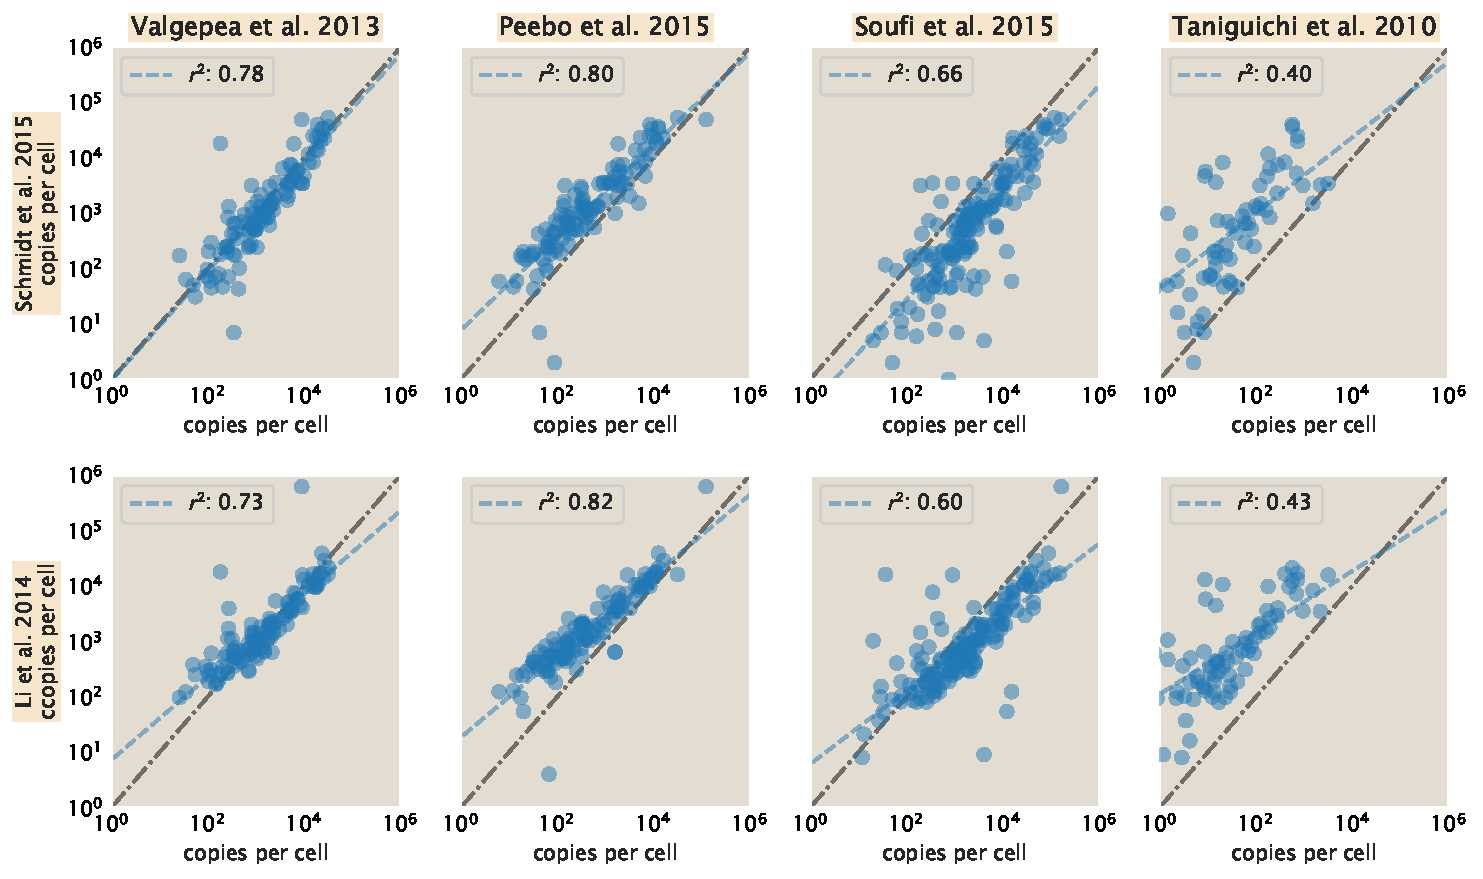
\includegraphics[width=1\textwidth]{../../figures/dataset_correlations.pdf}
  \caption{}
  \label{fig:dataset_correlations}
\end{figure}

\begin{figure}[H]
		\centering
    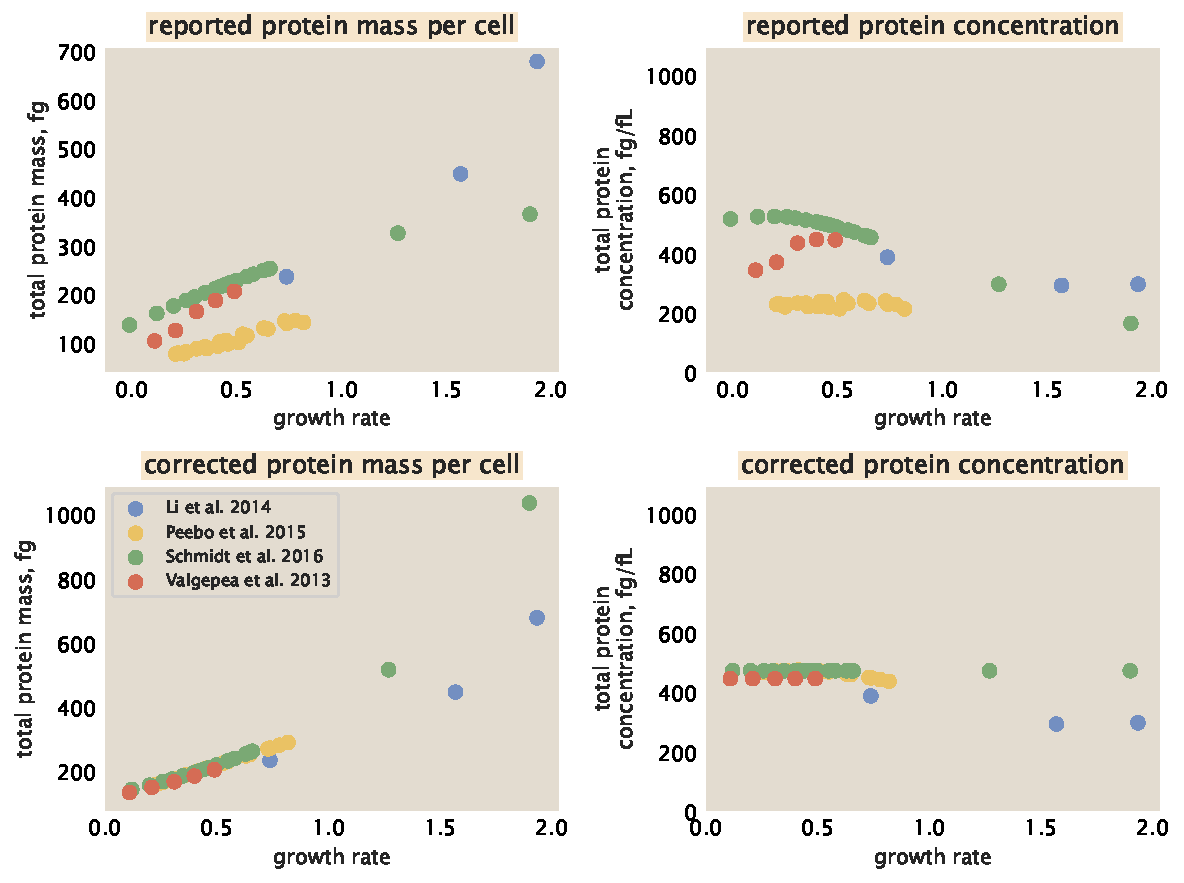
\includegraphics[width=1\textwidth]{../../figures/dataset_corrections.pdf}
  \caption{}
  \label{fig:dataset_correlations}
\end{figure}


\section{Adjustments to Copy Number Data.}

% NB: need to make summary figure with 2x2 panels; top row A) reported total protein per cells
% B) protein concentration. bottom row, C) new total protein mass per cell,
% C) new protein concentration.

% NB: It may be helpful to appeal to the 'classic growth laws' early on in this text
% as a rational to guide thinking with expections about total cell mass, cell volume w.r.t.
% growth rate.

The datasets encompass a range of bacterial growth conditions,  different {\it
e. coli} strains, and for those that report quantities on a cell basis,
different methods to normalize  by  cell count and volume. It was therefore
important to consider if certain discrepencies exist across the data and whether
these might be reasonably dealt with to make the compilated dataset internally
consistent. - give reference to what was done in example of yeast proteome data
corrections. However, given the work of [cite] and others, there are
well-documented expectations about how characteristics such as total protein
mass per cell and cell volume  should scale with growth rate. We were therefore
inclined to only renormalize data in a  way  that took into account such
expectations. Figure \ref{} shows the total protein  mass reported as a function
of growth rate for each experiment. Indeed, with the exception of the work of
Peebo et al., the total mass per cell is generally consistent as a fuction of
growth rate, and provide some confidence in such an approach.

In the remainder of this section we describe the rescaling that was done to each
dataset, with a particular focus on correcting for discrepencies in cellular
protein concentration, which may reflect differences in protein extraction
efficiency. It is important to note that with the exception of the work from
Peebo {\it et al.} (which is discussed more below), any rescaling is only
performed within the data of individual authors and not performed globally. We
felt this was important in order not to bias any individuals' work since we lack
any true standard of protein abundance.

% for differences in
% cellular protein concentration within each inidividual dataset. This  strategy
% was already applied in the work of Schmidt et al., in particularr due to
% concerns  over lower protein extraction efficiency in growth conditions like
% stationary phase.  However, another complicating factor that became apparent is
% a descrpency in expected versus reported cell volume that required additional
% care and is further described below. Lastly, the  data from Peebo {\it et al.}
% required additional care due to a lack quantities on a cell basis, and we
% consider this work seperately.


\subsection{Corrections to Enforce a Consistent Cellular Protein Concentration}

% NB: It may be useful to note that none of this should have any effect on the relative
% abundances found in each dataset.

One parameter that we do not expect to change substantially across growth
conditions is cellular protein concentration. As a general rule of thumb, we
expect an {\it e. coli} cell to have about 30\% dry mass, with about 55\% of
this expected from protein. With a density of about 1.1 g/ml, we find that the
protein concentration in a cell should be approximately 180 fg/fL.  The cellular
density and dry mass are essentially fixed, with the fraction of cellular
protein varying from [X-Y; refs??]. Hence,  this parameter provides a useful
reference point that datasets should agree on.  Indeed, out of concern over
differences in protein extraction efficiency in growth phases like stationary
phase, Schmidt {\it et al.} applied a correction to their measured protein
abundances to ensure cellular protein concentrations were internally consistent.


From the work of Schmidt {\it et al.} they reported an ability to consistently get high
protein yield from cells grown in M9 minimal media supplemented with glucose. In order
to account any protein loss during extraction, they use their measured protein concentration
from this sample as a reference for which total protein concentration in all other growth
conditions should match. This is shown in Figure \ref{}A. One challenge in
performing this calculation is that cell volume must be known; the authors use
volumes that were  measured by flow cytometry in previous work [cite]. These
volumes are shown in Figure \ref{}B. While it is difficult to assess the
accuracy of these numbers, we find them to be quite inconsistent with the
expected scaling that is reported by Taheri-Araghi {\it et al.} (2015),
carefully
measured as a function of growth rate [and other work?].

In addition,  since cell volume was not determined in all studies, and to be
consistent throughout, we instead use the predicted cell volumes from
Taheri-Araghi {\it et al.}. Dealing with each dataset seperately, we apply
correction  factors to correct for discrepencies in protein concentration across
the different growth conditions considered [NB: I wonder if in these other
datasets, the more appropriate thing to do is match to the average measured
protein concentration]. Specifically, the scaling factor $\phi$ is given by,

\begin{equation}
\phi  =  \frac{P_i}{V_i} \cdot [P]_r
\end{equation}

where $P_i$ is the total protein mass in conditino $i$, $V_i$ is the estimated cell volume, and $[P]_r$ is
the reference protein concentration (i.e. growth in  glucose for the Schmidt data).


\subsection{Peebo {\it et al.}: Conversion from copies/ fL to copies per cell}

In the work of Peebo {\it et al.}, the authors only report protein concentration.
In  order to determine protein per cell, we multiple these concentrations by
expected cell volumes  using the predictions from  Taheri-Araghi {\it et al.} This is
shown in Figure \ref{}A, where we see that reported mass is substantially lower than
the other work considered here; as well as work from others [Sinauer, 1990].

Indeed, both Schmidt {\it et al.} and Li {\it et al.} reported a total protein mass of about
250 fg per cell at a growth rate of about $\lambda \approx 0.5 hr^{-1}$ ( M9
minimal media with glucose and MOPS minimal media, respectively). Given this
descrepency, in addition to requiring that cellular protein concentration be
internally consistent across the growth conditions they reported on, we also
required that total cellular mass be consistent with the work Schmidt {\it et al.} and
Li {\it et al.} This amounted to performing a linear regression between total protein
mass and growth rate, and using this to scale the Peebo {\it et al.} dataset according
to this trend.


 % cell biology by the numebrs: Overall macromolecular composition of an average
 % E. coli cell in aerobic balanced growth at 37°C in glucose minimal medium,
 % with doubling time of 40 minutes and 1 pg cell wet weight (≈0.9 μm^3 cell
 % volume). Adapted with modifications from F. C. Neidhardt et al., “Physiology
 % of the bacterial cell”, Sinauer, 1990 (BNID 104954). Modifications included
 % increasing cell dry weight from 284 fg to 300 fg and total cell mass from 950
 % to 1000 fg as

%
\newpage
\section{Translation-dependent limits on the rate of cell division.}

Here we consider the hypothesis that synthesis of ribosomes represents the
rate-limiting process of cell division. In addition, we consider how a cell
might try to achieve this rate of growth and the potential implications on the
required ribosomal content of the cell.

\subsection{Maximum possible growth rate is set by the time to make a ribosome.}

\marginnote{\small{NB: I wonder if this should also account for the time to make the other ribosomal components}}

Ribosomes take a unique position among proteins due to their role in
replicating the entire pool of cellular proteins, including themselves. In
order for a cell to maintain its copy number of ribosomes during division into two
daughter cells, each ribosome must make all the protein subunits for a second
ribosome.  Since the  mass of a single ribosome is about 2.5 MDa, with about 2/3
RNA and 1/3 protein, each ribosome has to make about 800 kDa of protein. In {\it
E. coli}, this corresponds to 7459 amino acids. At a maximal rate of 20 amino
acids per second, this would take just over 6 minutes.  This time for the
synthesis of a ribosome sets a firm time limit on how fast a cell can double
itself. Irrespective of the absolute number of ribosomes in a cell, the time to
double their number is given by our calculation above. This contrasts with other
proteins, where the simple solution to making more proteins is to apparently
devote more ribosomes to their synthesis.


\subsection{Translation-dependent maximum rate of growth is set by the number of
ribosomes.}

While the inability to parallelize ribosome synthesis sets an inherent speed
limit, this represents a somewhat unachievable rate since the ribosomes must
spend some of their time also doubling all the other proteins present in the
cell. A translation-limited rate of growth will then be set by the time to
double the entire proteome. The only way to reach the minimum duplication time
set by the ribosome would be to increase the relative fraction of ribosomes.
This would effectively reduce the time needed to duplicate the non-ribosomal
proteins.

In order to understand the consequence of each ribosome having to duplicate
itself and devote time to double the remaining proteome, we will make use of a
toy model. Specifically, lets consider a hypothetical cell that consists of two
species of protein, R and P. Here R refers to ribosomes, with $R$ per cell, and
P reflects the remaining proteins in the cell with $P$ copies per cell. The time
$\tau$ needed to duplicate the entire proteome is simplly given by,

\begin{equation}
	\tau = \tau_R + \tau_P,
\label{eq:tau}
\end{equation}
where $\tau_R$ is the time to double a ribosome, while $\tau_P$ is the time
required to double the remaining proteome. While we found that $\tau_R$ is fixed
at about 6 minutes,  $\tau_P$  will depend on the number of ribosomes $R$ and
can be approximated by,

\begin{equation}
\tau_P = \frac{N_{aa}}{r_t \cdot R}.
\label{eq:tau_P}
\end{equation}
Here $N_{aa}$ refers to the total number of amino acids (aa) that must be translated,
while $r_t$ refers to the rate of translation, at about 20 aa /
sec. Finally, we can then calculate a translation-limited growth rate from,

\begin{equation}
\lambda_{\text{max}} =  \frac{ln(2)} {\tau}.
\end{equation}
Using Equation \ref{eq:tau_P} and \ref{eq:tau}, this becomes,
\begin{equation}
\lambda_{\text{max}} =  \frac{ln(2)} {\tau_R + \frac{N_{aa}}{r_t \cdot R}}.
\label{eq:lambda_max}
\end{equation}
 We can see from this that the only way to increase the translation-limited
growth rate would be to make more ribosomes, or if it were possible, to decrease the
number non-ribosomal proteome.

% Lastly, we can also consider how $\lambda_{\text{max}}$ will vary with the
% ribosomal mass fraction, denoted by $\Phi_R$. An amino acid has an average molecular weight
% of 110 Da, and the approximate non-ribosomal mass will be given by $110 \text{ Da} \cdot (N_{aa}/ N_A)$.
% Here, $N_A$ is Avagadros number. The ribosomal mass is similarly given by $800 \text{ Da} \cdot (R/ N_A)$.
% Therefore we can rewrite Equation \ref{eq:lambda_max} in
% as the ribosomal mass fraction,
%
% M_nr = (N (molecules) / (N_A molecules/mol)) * 110 g/mol
%
% M_r =  (R  / (N_A molecules/mol))) *  800 g/mol
% R = N_A * M_r / 800
% Naa = N_A * M_nr / 110
%
% Phi = M_r / (M_r + M_nr)
% = R*800 / (R*800 + Naa * 110)
% Phi / (R*800) = 1/(1 + (Naa*110)/ (R*800))
%
% (1 + (Naa*110)/ (R*800)) = (R*800)/ Phi
% (Naa*110)/ (R*800)  = (R*800)/ Phi  - 1
% (Naa/R) = (800) * ((R*800)/ Phi  - 1) /110
%
% R/ Phi = (R*800 + Naa * 110) /

\marginnote{\small{NB: I should also write this in terms of ribosome mass fraction.}}

Next, lets consider some representative values of $R$ and $N_{aa}$ and plot
$\lambda_{\text{max}}$. From Schmidt {\it et al.}, cells growth in glucose were
found to have 214 fg of non-ribosomal  protein mass. This corresponds to about
1.17 x 10$^9$ amino acids. We also estimate a  ribosomal copy number, $R$ =
20,656 per cell based on the mean copy number of individual subunit copy
numbers. Using Equation \ref{eq:lambda_max}, this corresponds to a maximum
growth rate of 0.78 hr$^-1$, versus the measured rate of 0.58 hr$^-1$.

As we noted earlier, the only way to divide faster than this is to make more
ribosomes. One additional difficultly that arises is that in order for a cell to
add proteins, it likely will need to increase in size. This may then require
that other proteomic proteins also increase in proportion. However, to keep our
problem simple, lets proceed with the simplifying assumption that the value of
$N_{aa}$ is sufficient to build a cell irrespective of the number of ribosomes.
This in effect provides a lower bound on the total proteomic content at faster
growth rates. In Figure \ref{} we plot the translation-limited growth rate
$\lambda_{\text{max}}$ as a function of ribosome copy number per cell. While indeed,
the maximum attainable growth rate is that set by the time to make a ribosome,
it could only be reached if the number of ribosomes was increased about 100 fold.

As a last consideration, one observation is the apparently linear
increase in the fraction of ribosomal mass. This, along with the dramatic
scaling in ribosomal copy number, are particularly relavent to the
phenemonlogical growth laws reported by others on how cell size and cell mass
scale with growth rate in bacteria.  This will require further thought, but as a
starting point, we can estimate the lower bound in cell volume as a function of
the number of ribosomes through the following assumptions:  mass density of 1.1
g/ml, a dry mass of 30\% that consists of only protein and RNA.  This is shown
in  Figure \ref{}.

\subsection{Growth only appears Translation-limited in rich growth media.}

\marginnote{\small{NB: A better way would be to directly calculate the number of
aa from proteomic sequences and copy number.}}

With some expectation on the maximum growth rate achiveable as a function of
ribosomal content, lets now take a look a look at how our experimental data
compares. To simplify our calculations, we will approximate the number of amino
acids that must be translated from the reported protein mass and 110 Da for the
average molecular weight of an amino acid. Using Equation \ref{eq:lambda_max},
we can then calculate the maximum rate of growth under translation limitation.
In Figure \ref{}A we plot maximum growth under translation limitation against
the measured growth rates, while in Figure \ref{}B we plot the cell cycle time
that would be associated with these growth rates. The shaded regions identify
the regions that should not be attainable with a translation rate of 20 aa/sec.
From these two plots, it appears to we are only translation-limited
in rich media (data points with growth rates great than 1 hr$^{-1}$ in Figure \ref{}A)).
Though it should be noted that a more careful  calculation of the maximum
tranlation time suggested by Equation \ref{eq:lambda_max} needs to be
undertaken.

\marginnote{\small{NB: There is something weird about the fraction of ribosomal
protein in Peebo, Valgepea; it is higher, and also higher than found in Scott
{\it et al.}  - is it real??}}

From Figure \ref{}B, it is apparent that at the slower growth rates, the cell
cycle  time is indeed much longer than might have been expected given a
translation rate of 20 aa/sec. We can actually infer what the apparent or
effective translation is given the observed growth rate and show this in Figure
\ref{}.  Interestingly, these translation rates are in good agreement with those
measured in Dai {\it et al.}, though that work also suggets that the fraction of
active ribosomes may decrease in poor nutrient conditions, further suggesting
that under a certain regime cells may not be utilizaing their full ribosomal
capacity (i.e. not translation-limited).







\end{document}
